\documentclass[11pt,a4paper]{report}
\usepackage[tmargin=1cm,rmargin=1in,lmargin=1in,margin=0.85in,bmargin=1cm,footskip=.2in]{geometry}

\title{REAL112-1 24H - Fysikk\\Obligatorisk innlevering 4}
\author{Casper Eide Özdemir-Børretzen}
\date{}

\makeatletter
\newcommand{\institle}{\@title}
\newcommand{\insauthor}{\@author}
\newcommand{\insdate}{\@date}
\makeatother

\usepackage[utf8]{inputenc}
\usepackage[T1]{fontenc}
\usepackage{ulem}           % Double underline
\setlength{\parindent}{0pt}
\usepackage[fleqn]{amsmath}
\usepackage{amssymb}
\usepackage{pdfpages}
\usepackage{enumitem}
\usepackage{circuitikz}

\newcommand{\opg}[1]{\subsection*{Oppgave #1}}
\newcommand{\opgd}[1]{\item[#1)]}

\begin{document}
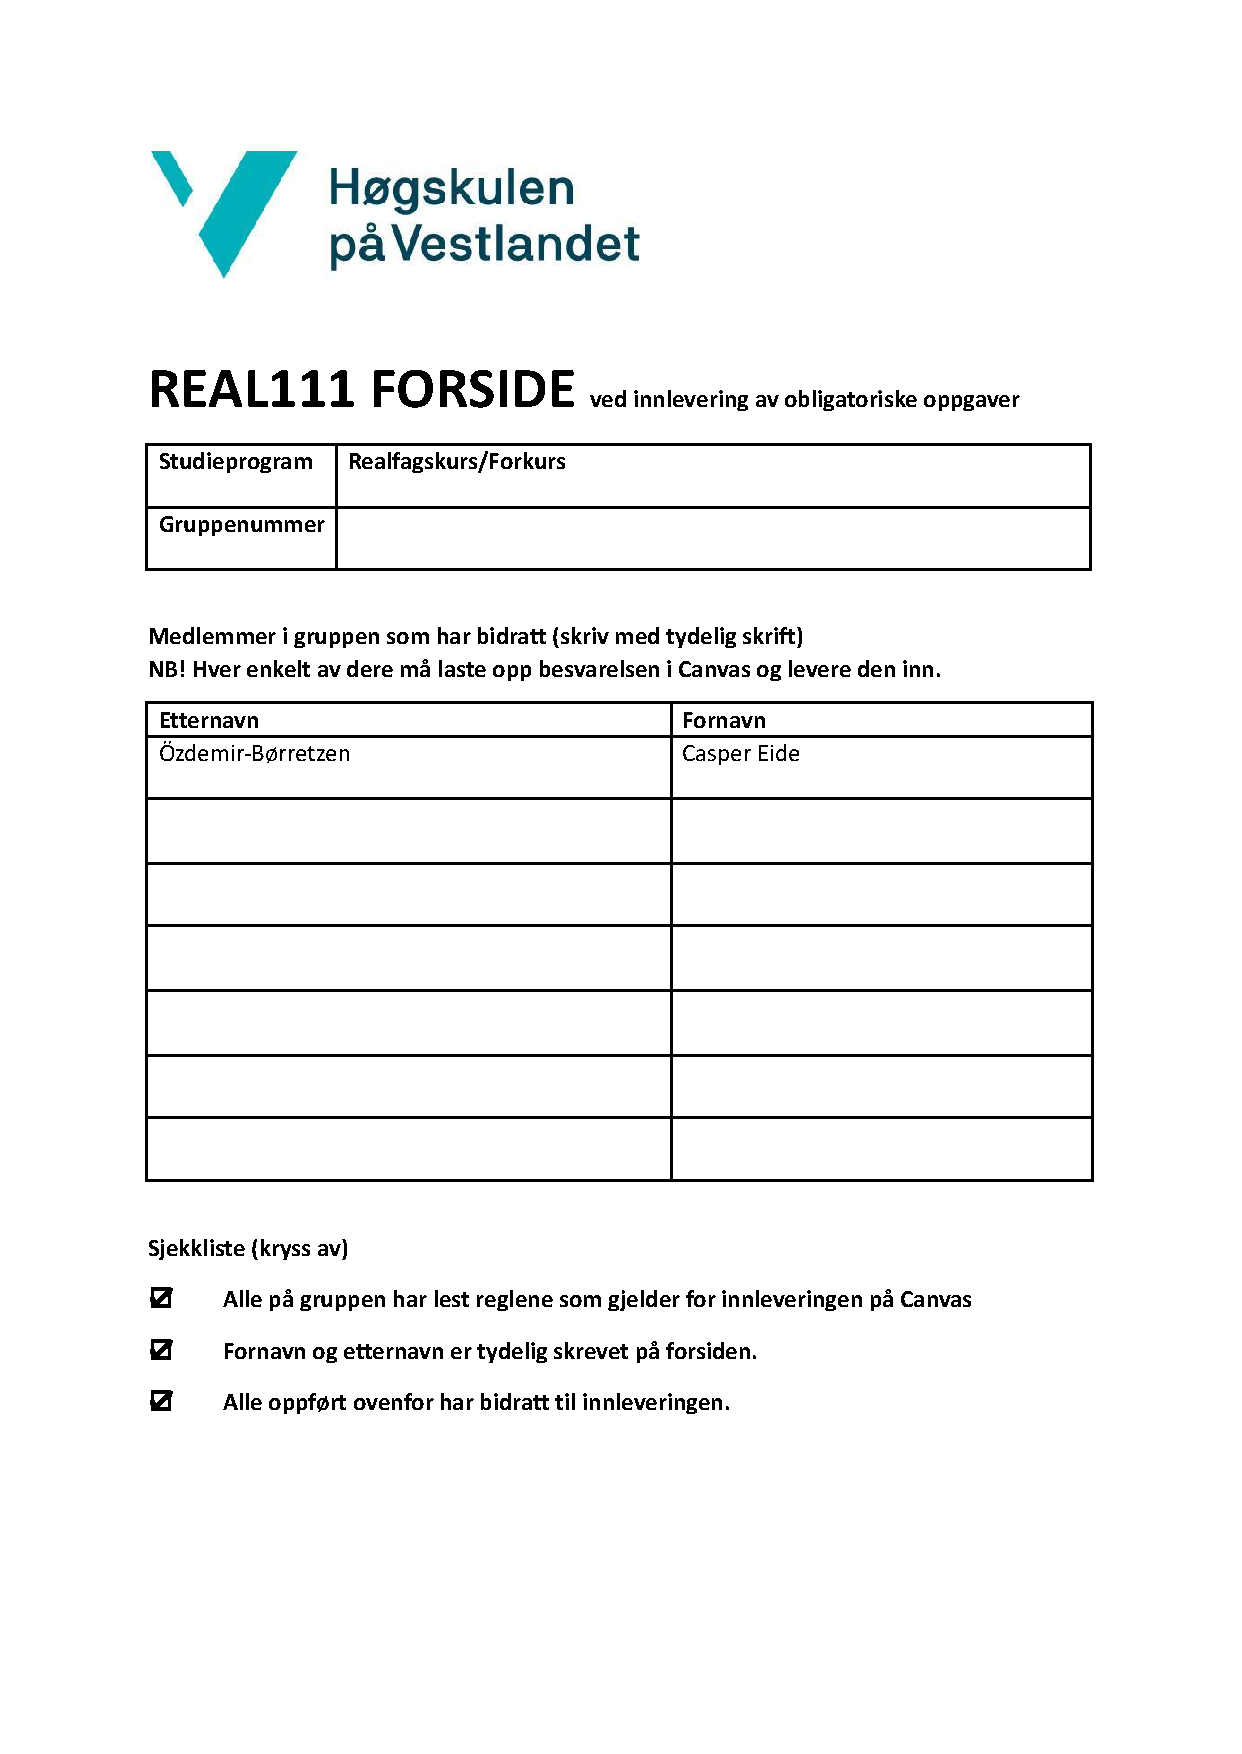
\includepdf[pages={1}]{real111-forside.pdf}

\opg{1}
\begin{enumerate}[leftmargin=*,itemsep=2cm,labelsep=2em,label=\alph*)]
\opgd{a} \ \\

\begin{circuitikz}
\draw (0,2) to[battery1, l_={$U_p$}] (0,-2);
\draw (0,2) to[lamp, name=lamp, l^={$U_L = 6,0\ V$}] (8, 2)
\draw (lamp.south) node[below] {$6,0\ V\ /\ 9,0\ W$}
\draw (8,2) -- (8,-2)
\draw (8,-2) -- (7,-2)
\draw (0,-2) -- (1,-2)
\draw (1,-1) -- (1,-3)
\draw (7,-1) -- (7,-3)
\draw (1,-1) to[R, l^={$R_1 = 10\ \Omega$}] (7,-1)
\draw (1,-3) to[R, l_={$R_2 = ?$}] (7,-3)
\end{circuitikz}

\begin{align*}
&\mathcal{E} = 7,5\ V = R_i I + R_y I &&$der $ U_p = R_y I $ og $ $R_i = 0\\\\
&U_P = \mathcal{E} = 7,5\ V
\end{align*}

\opgd{b}
\begin{align*}
&P = UI$$\\\\
&I = \frac{P}{U} = \frac{9,0\ W}{6,0\ V} = \uuline{1,5\ A}
\end{align*}
\end{enumerate}

\newpage

\opg{1}
\begin{enumerate}[leftmargin=*,itemsep=2cm,labelsep=2em,label=\alph*)]
\opgd{c}
\begin{align*}
&U_P = U_L + U_R\\\\
&U_R = U_P - U_L = 7,5\ V - 6,0\ V = 1,5\ V\\\\
&R_R = \frac{U_R}{I} = \frac{1,5\ V}{1,5\ A} = 1,0\ \Omega\\
\end{align*}

Den totale resistansen for de to parallellkoblede motstandene er $1,0\ \Omega$.\\

\begin{align*}
&\frac{1}{R_R} = \frac{1}{R_1} + \frac{1}{R_2}\\\\
&\frac{1}{R_2} = \frac{1}{R_R} - \frac{1}{R_1}\\\\
&\frac{1}{R_2} = \frac{1 \cdot 10}{1,0 \cdot 10}\  \Omega - \frac{1}{10}\ \Omega = \frac{9}{10}\ \Omega\\\\
&\left( \frac{1}{R_2} \right)^{-1} = \left( \frac{9}{10} \right)^{-1}\ \Omega = 1,11111\ \Omega\\\\
&\uuline{R_2 = 1,1\ \Omega}
\end{align*}
\end{enumerate}

\newpage

\opg{2}
\begin{enumerate}[leftmargin=*,itemsep=2cm,labelsep=2em,label=\alph*)]
\opgd{a}
\begin{align*}
&m = 37 \cdot 10^3\ kg\\\\
&h = 735\ m\\\\
&P = E/s = \frac{mgh}{s} = \frac{37 \cdot 10^3\ kg \cdot 9,81\ N/kg \cdot 735\ m}{s} = 266782950\ J/s\\\\
&P_{tot} = \frac{P \cdot (60 \cdot 60 \cdot 24 \cdot 365)\ s}{3600\ s} = 2,33702 \cdot 10^{12}\ Wh\\
\end{align*}

Den teoretisk største effekten vannkraften kan levere er \uuline{$267\ MJ$ per sekund}, som ville gitt \uuline{2,34 terrawattimer energi per år.}

\opgd{b}
\begin{align*}
&\eta = \frac{220\ MW}{267\ MW} = 0,82397\\\\
&\uuline{\eta = 82\ \%}
\end{align*}

\opgd{c}
\begin{align*}
&\frac{220 \cdot 10^6\ J/s \cdot (60 \cdot 60 \cdot 24 \cdot 365)\ s}{3600\ s} = 1927,2\ GWh\\\\
&\frac{1027\ GWh}{1927,2\ GWh} = 0,5329\\
\end{align*}

\uuline{Med effekten $220\ MW$ og en årsproduksjon på $1027\ GWh$ kan det antas at kraftverket er på $53\ \%$ av tiden.}
\end{enumerate}

\newpage

\opg{3}
\begin{align*}
&\mathcal{E} = 12,0\ V\\
&R_i = 0,30\ \Omega\\
&R_a = 0,50\ \Omega\\
&R_{L1} = R_{L2} = R_{L3} = 21,0\ \Omega\\
&R_{L4} = 13,0\ \Omega
\end{align*}
\begin{enumerate}[leftmargin=*,itemsep=2cm,labelsep=2em,label=\alph*)]
\opgd{a}
\begin{align*}
&\frac{1}{R_{par}} = \frac{1}{R_{L1}} + \frac{1}{R_{L2}} + \frac{1}{R_{L3}} = \frac{1}{21,0\ \Omega} + \frac{1}{21,0\ \Omega} + \frac{1}{21,0\ \Omega}\\\\
&\left( \frac{1}{R_{par}} \right)^{-1} = \left( \frac{3}{21,0\ \Omega} \right)^{-1}\\\\
&R_{par} = 7,0\ \Omega\\\\
&R_y = R_{L4} + R_{par} + R_a = 13,0\ \Omega + 7,0\ \Omega + 0,50\ \Omega\\\\
&R_y = 20,5\ \Omega\\
\end{align*}

\uuline{Resultantresistansen for lampene $L1$, $L2$ og $L3$ er $7,0\ \Omega$.}\\

\uuline{Resultantresistansen i den ytre kretsen er $20,5\ \Omega$.}

\opgd{b}
\begin{align*}
&\mathcal{E} = R_i I + R_y I = I ( R_i + R_y ) &&| : (R_i + R_y)\\\\
&I = \frac{\mathcal{E}}{R_i + R_y} = \frac{12,0\ V}{0,30\ \Omega + 20,5\ \Omega} = \frac{12,0\ V}{20,8\ \Omega} = 0,57692\ A\\\\
&I = 0,58\ A\\
\end{align*}

\uuline{Amperemeteret viser $0,58\ A$.}

\end{enumerate}

\newpage

\opg{3}
\begin{enumerate}[leftmargin=*,itemsep=2cm,labelsep=2em,label=\alph*)]
\opgd{c}
\begin{align*}
&U_p = R_y I = 20,5\ \Omega \cdot 0,58\ A = 11,89\ V\\\\
&U_p = 11,9\ V\\
\end{align*}

\uuline{Polspenningen er 11,9\ V.}

\opgd{d}
\begin{align*}
&P_{L4} = R_{L4} \cdot I^2 = 13,0\ \Omega \cdot 0,57692^2\ A = 4,33\ W\\\\
&U_{par} = R_{par} \cdot I = 7,0\ \Omega \cdot 0,57692\ A = 4,03844\ V\\\\
&P_{L1} = \frac{U_{par}^2}{R_{L1}} = \frac{4,03844^2\ V}{21,0\ \Omega} = 0,77662\ W\\\\
&P_{L1} = P_{L2} = P_{L3} = 0,78\ W\\
\end{align*}

\uuline{Lampene $L1$, $L2$ og $L3$ har en elektrisk effekt på $0,78\ W$ og $L4$ har en effekt på $4,33\ W$.}

\opgd{e}
Dersom lyspæren $L1$ skrus ut vil lysstyrken i $L2$ og $L3$ være samme som før, mens $L4$ vil lyse sterkere.

\opgd{f}
Ved kortslutning i $L1$ vil $L2$ og $L3$ slutte å lyse, og $L4$ vil lyse sterkere.

\end{enumerate}

\end{document}
